\chapter{Вынужденное движение}

Рассмотреть систему 2-го порядка, заданную дифференциальным уравнением:
\[
\ddot y + a_1 \dot y + a_0 y = u
\]

Воспользуемся Simulink схемой из прошлой лабораторной работы и 
немного изменим ее, добавив в нее блок выбора входного сигнала:

\begin{figure}[ht]
    \centering
    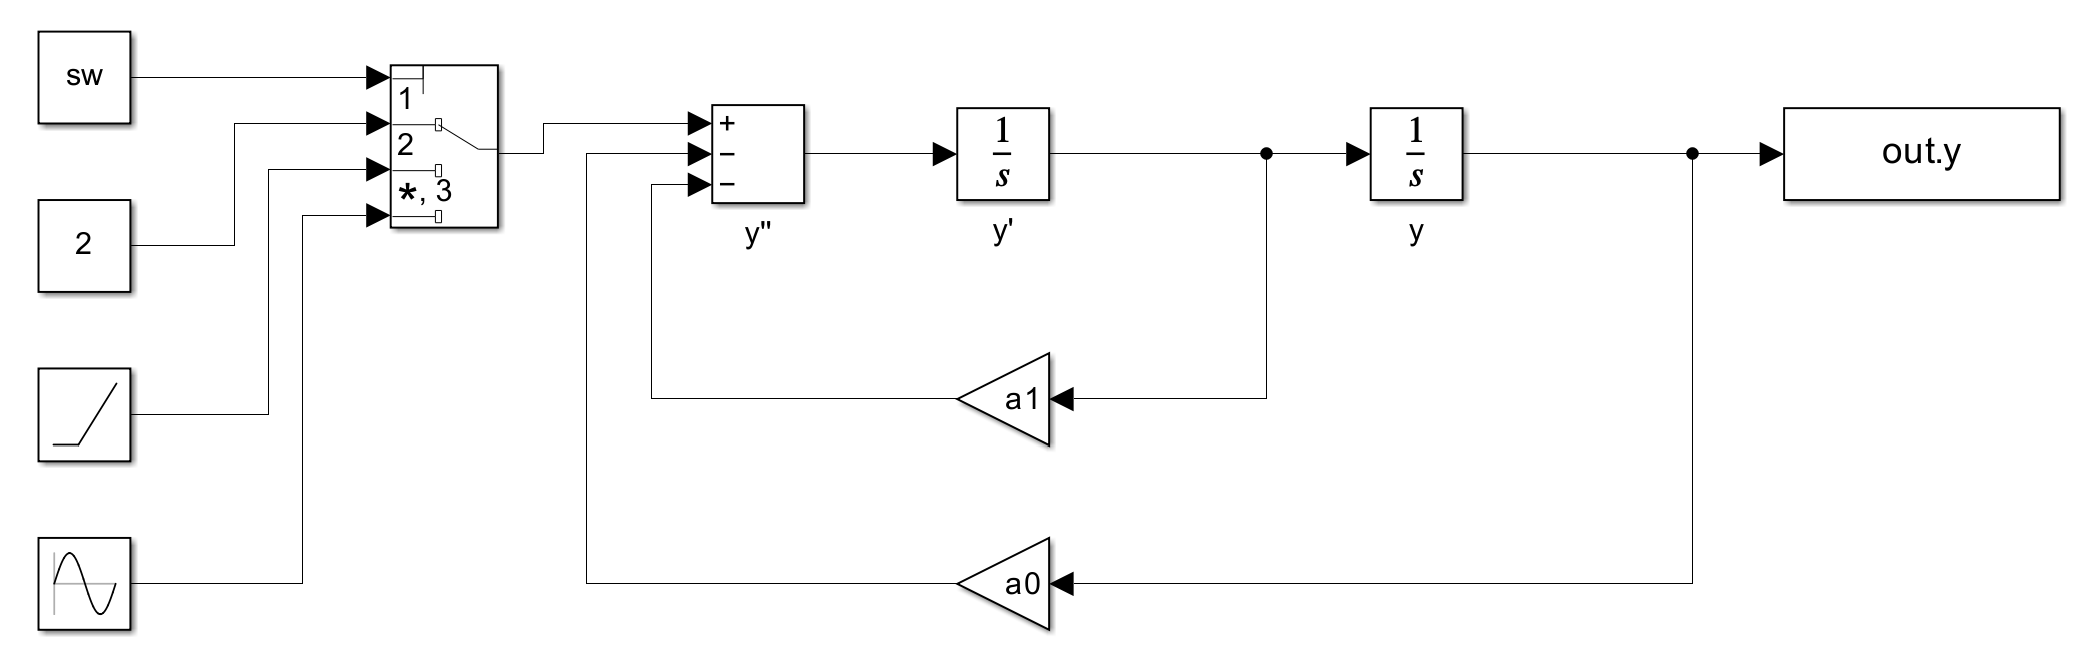
\includegraphics[width=1\textwidth, trim={0cm 0cm 0cm 0cm}]{../images/sim1}
    \caption{схема Simulink}
    \label{fig:sim1}
\end{figure}

Теперь возьмем коэффициенты $a_0$, $a_1$ из экспериментов 2-4 прошлой лабораторной
работы и проведем моделирование при 3-х начальных условиях:
\begin{enumerate}
    \item $y(0) = -1, \dot y(0) = 0$
    \item $y(0) = 0, \dot y(0) = 0$
    \item $y(0) = 1, \dot y(0) = 0$
\end{enumerate}

И 3-х входных сигналах:
\begin{enumerate}
    \item $u(t) = 2$
    \item $u(t) = 0.7t$
    \item $u(t) = \sin(7t)$
\end{enumerate}

\newpage
\section{$a_0 = 82.21,\, a_1 = 2.2$}

\begin{figure}[ht]
    \centering
    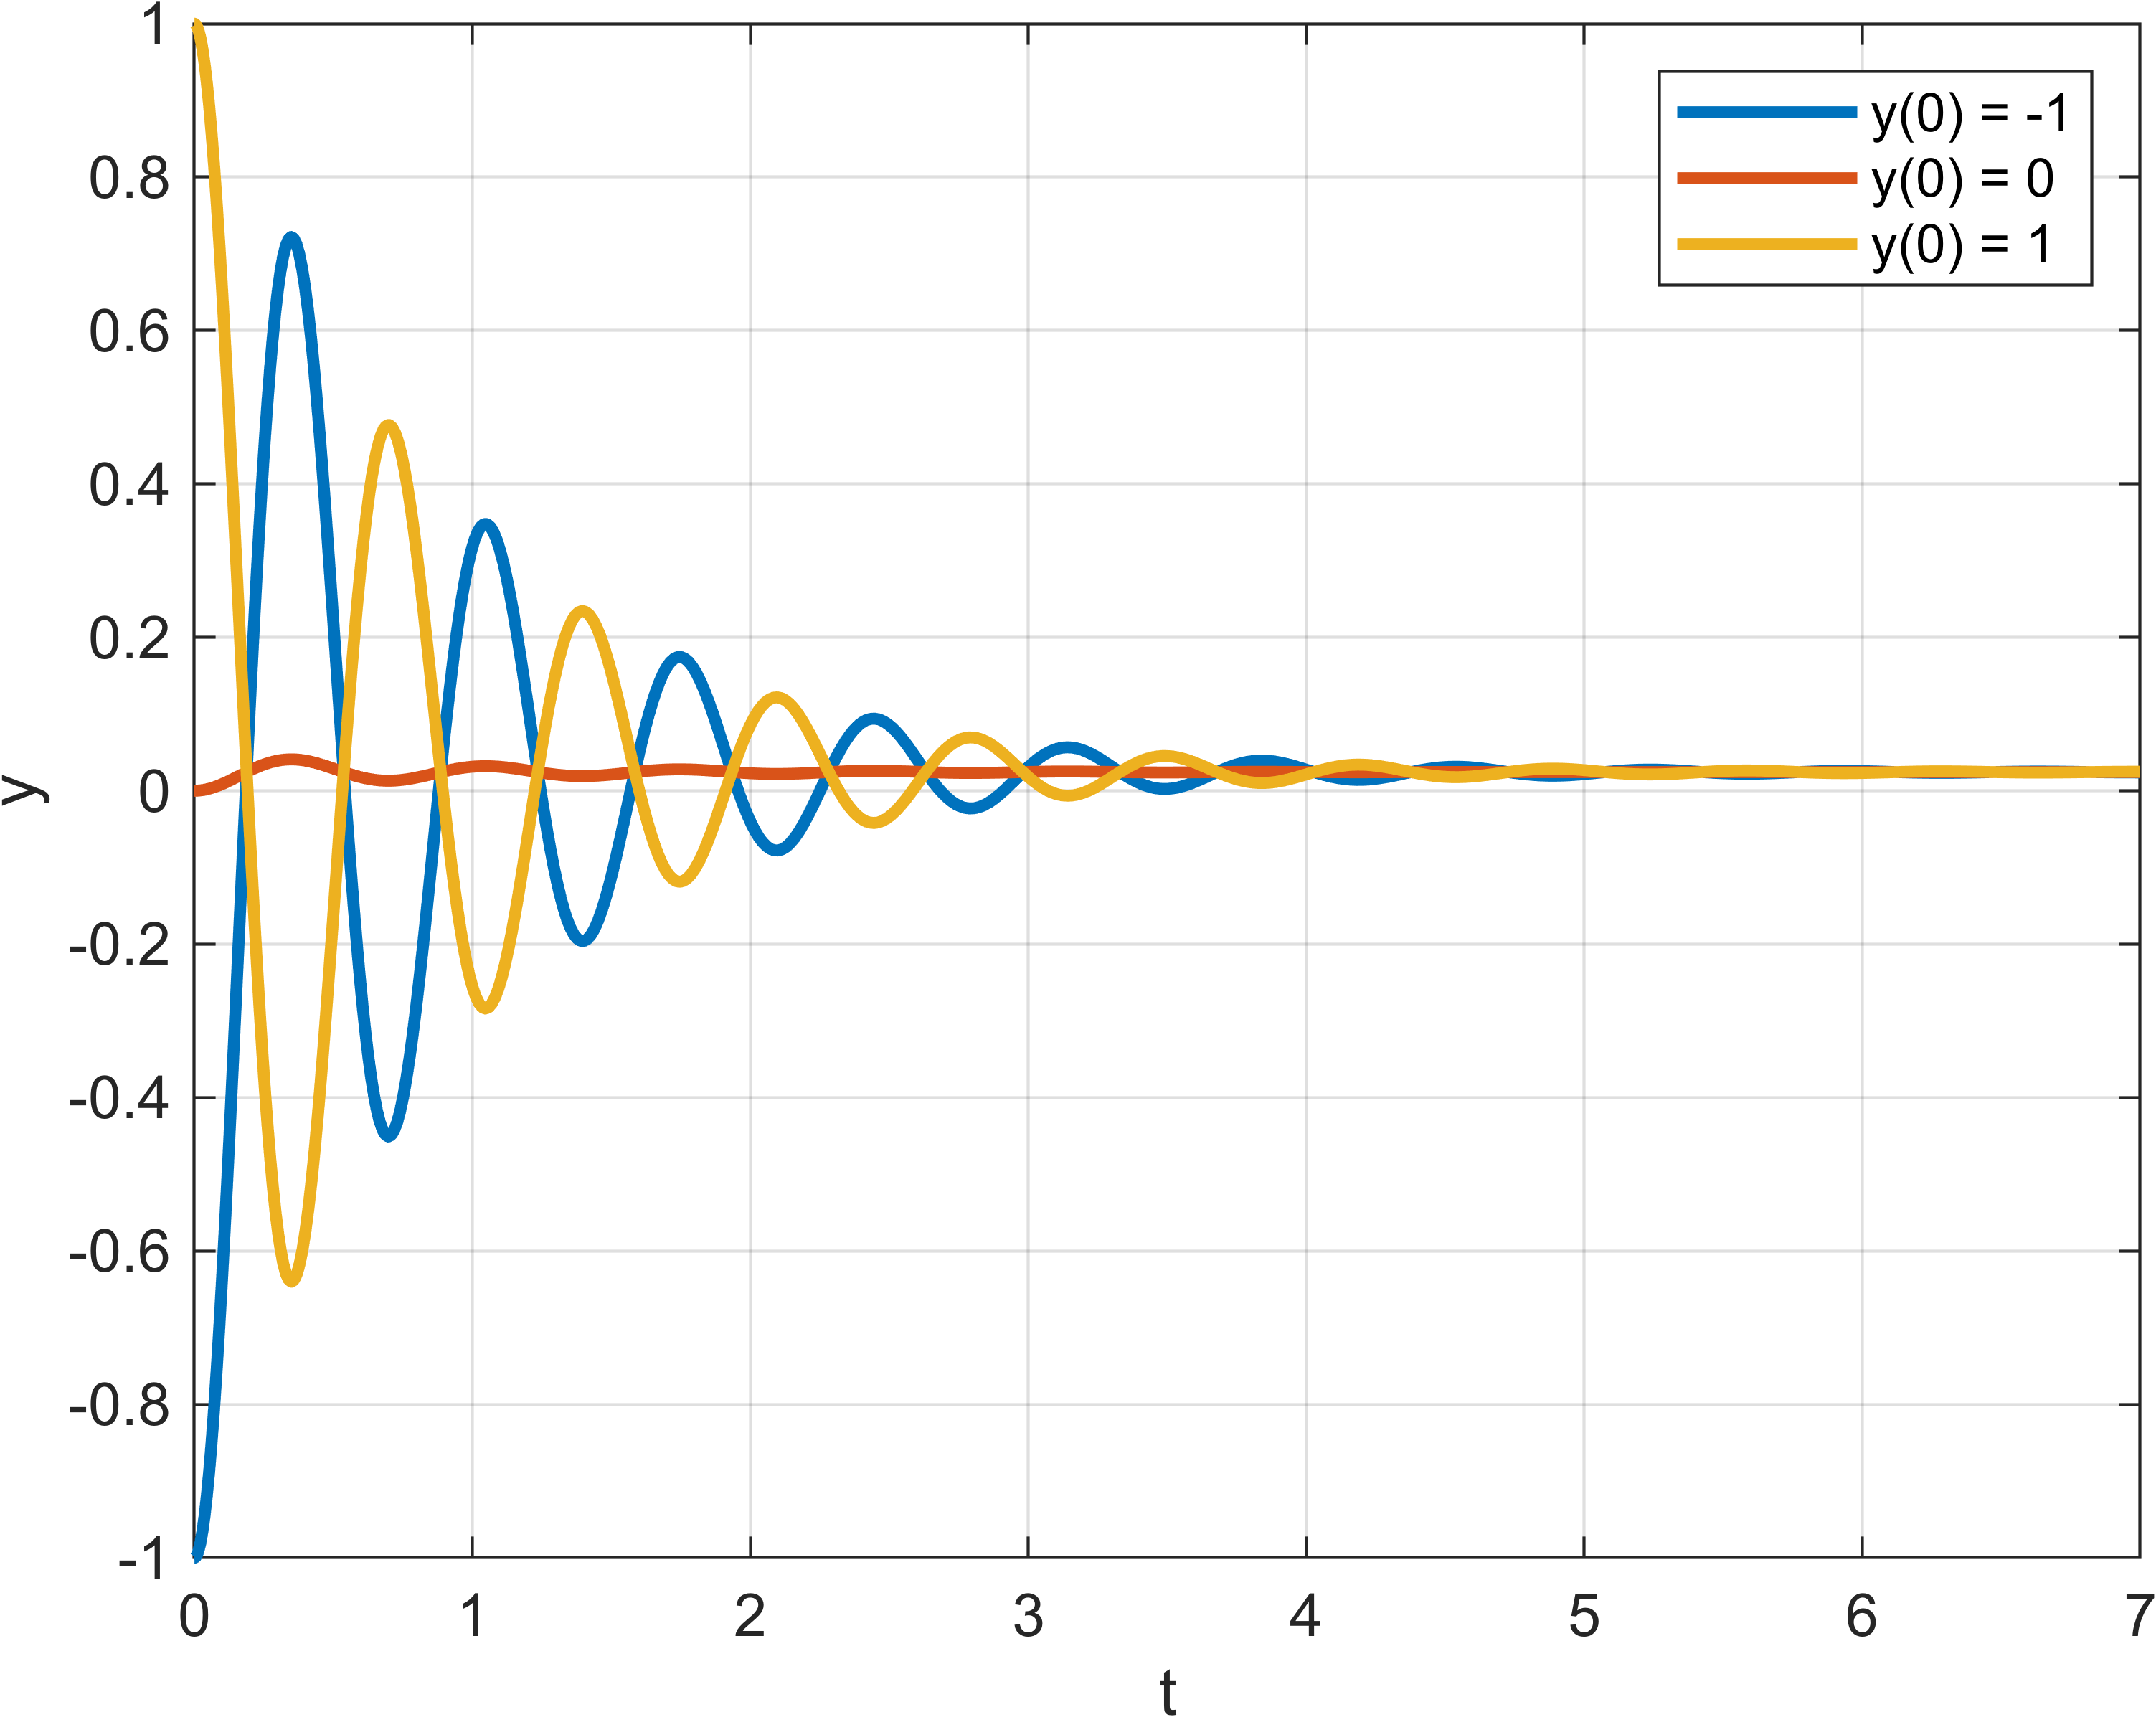
\includegraphics[width=0.7\textwidth, trim={0cm 0cm 0cm 0cm}]{../images/1_1.png}
    \caption{$u(t) = 2$}
    \label{fig:1_1}
\end{figure}

\begin{figure}[ht]
    \centering
    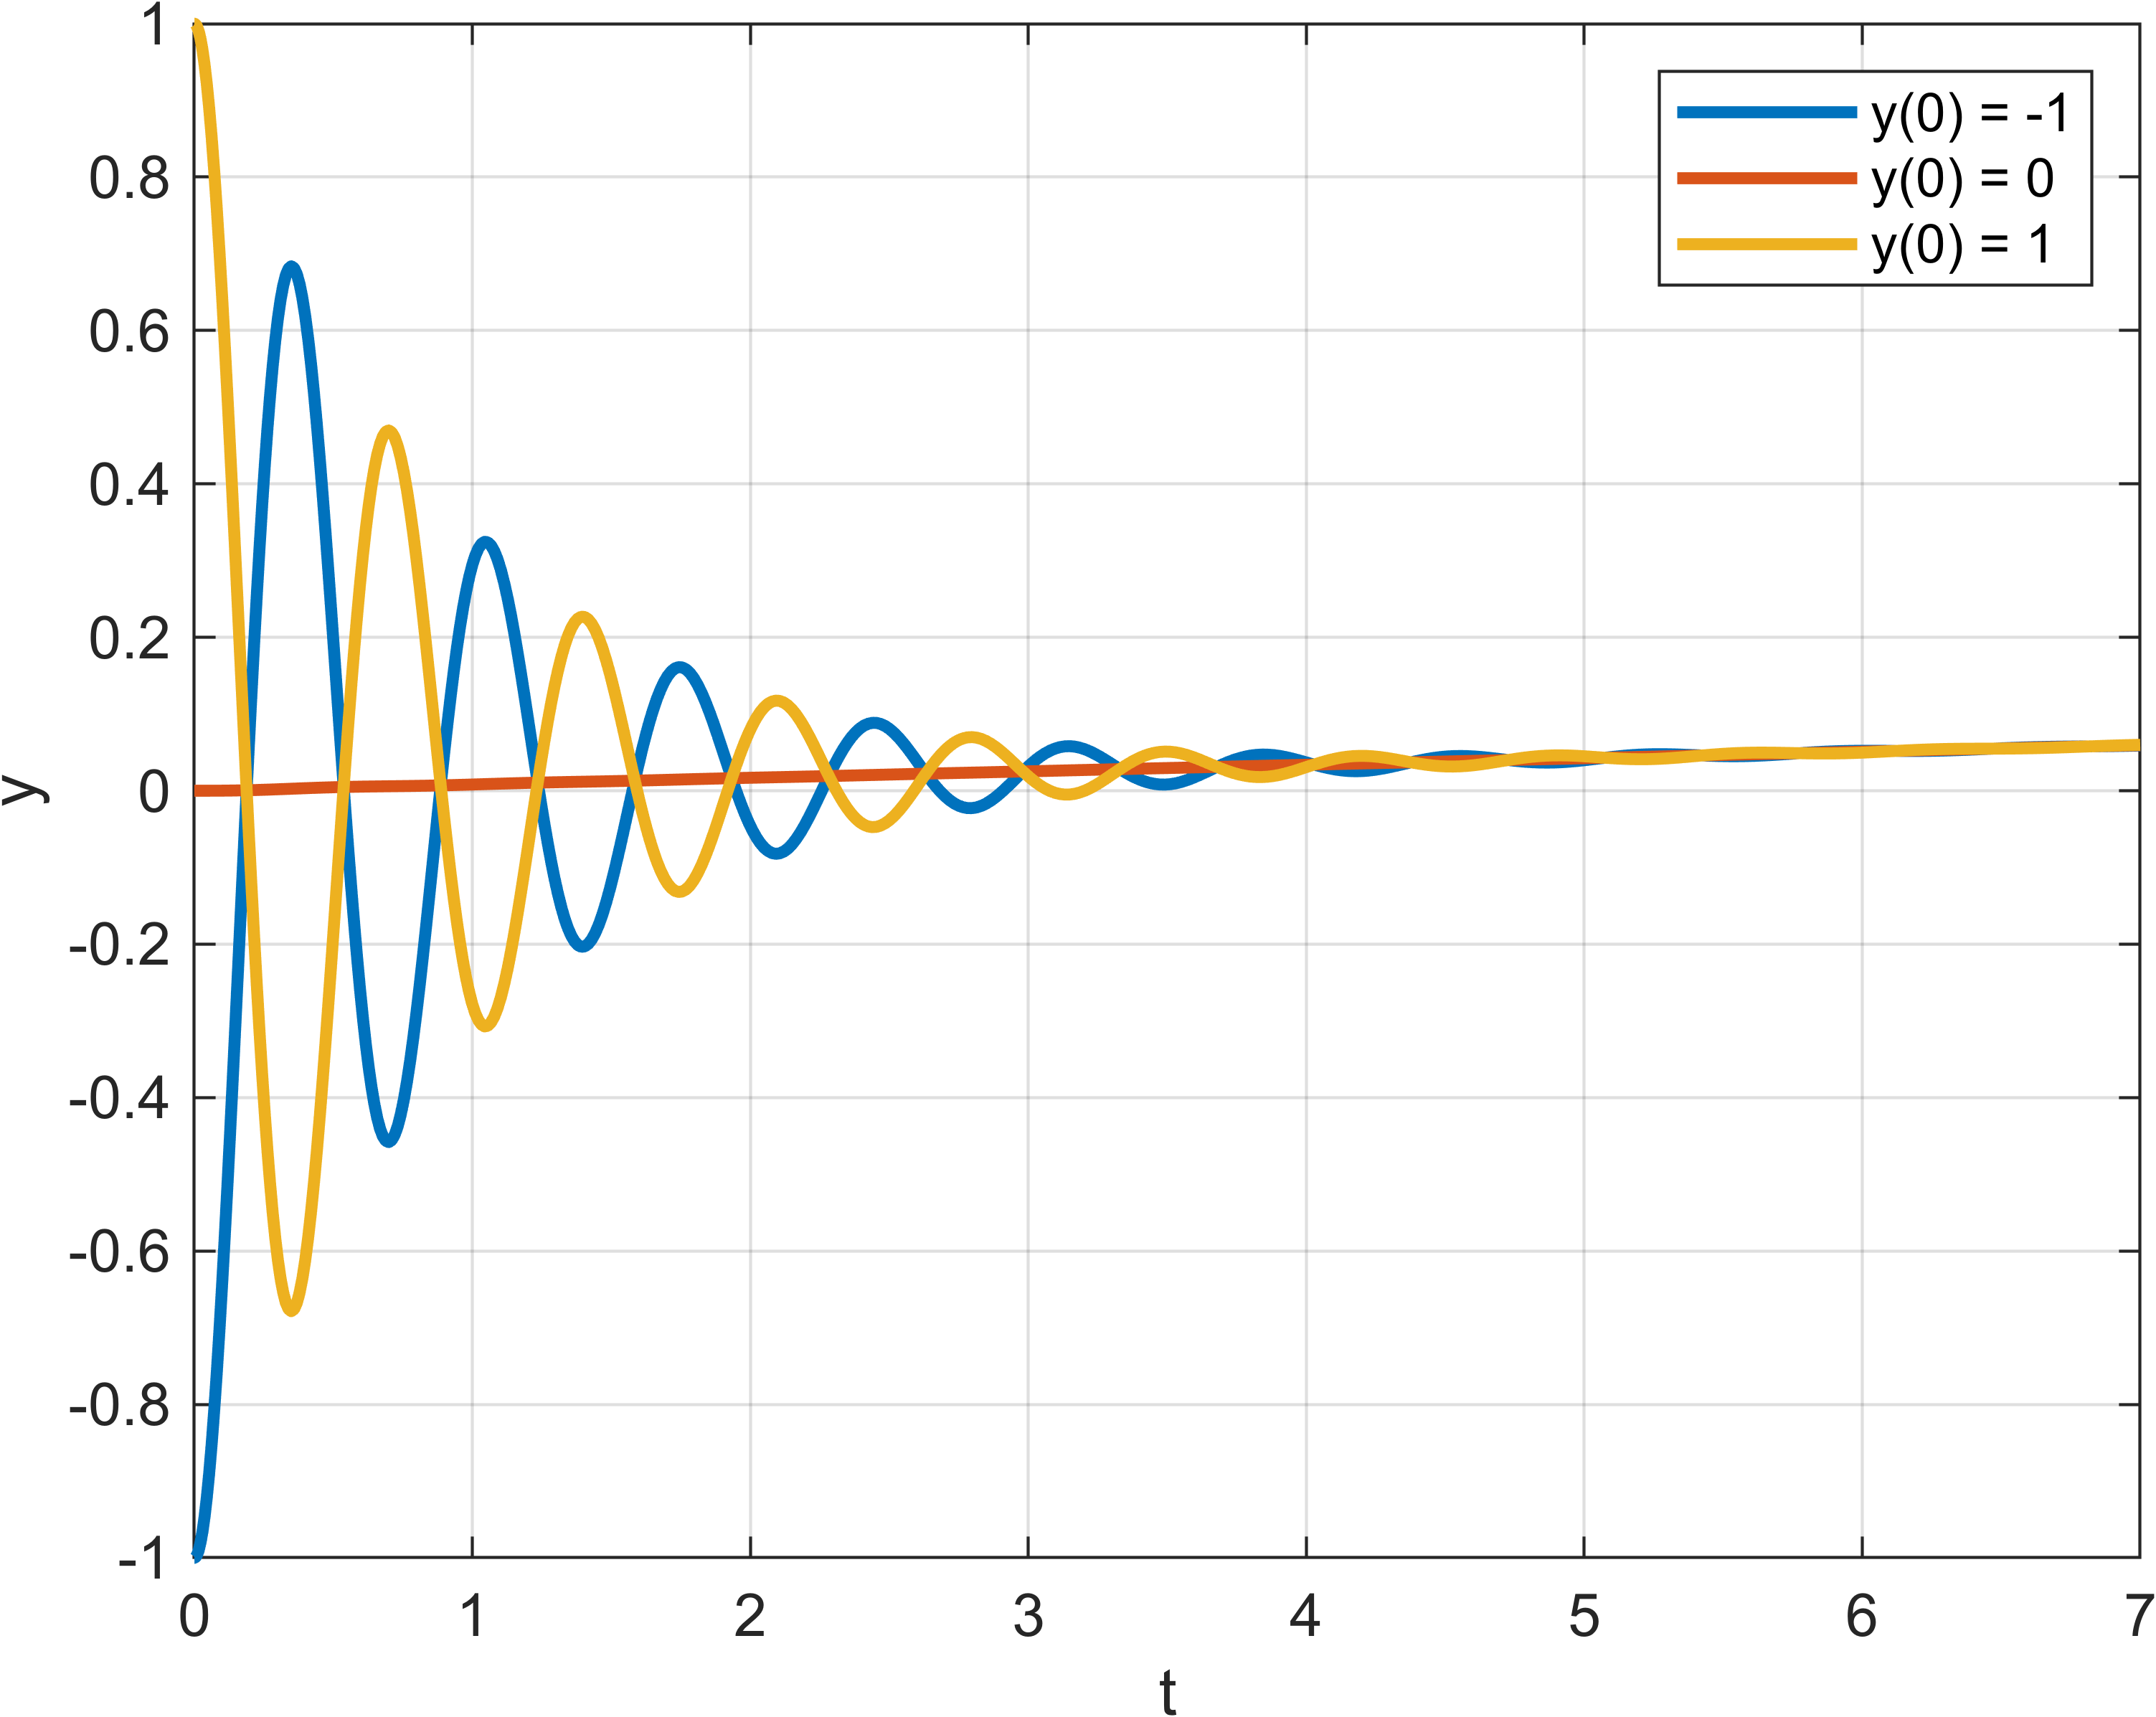
\includegraphics[width=0.7\textwidth, trim={0cm 0cm 0cm 0cm}]{../images/1_2.png}
    \caption{$u(t) = 0.7t$}
    \label{fig:1_2}
\end{figure}

\begin{figure}[ht]
    \centering
    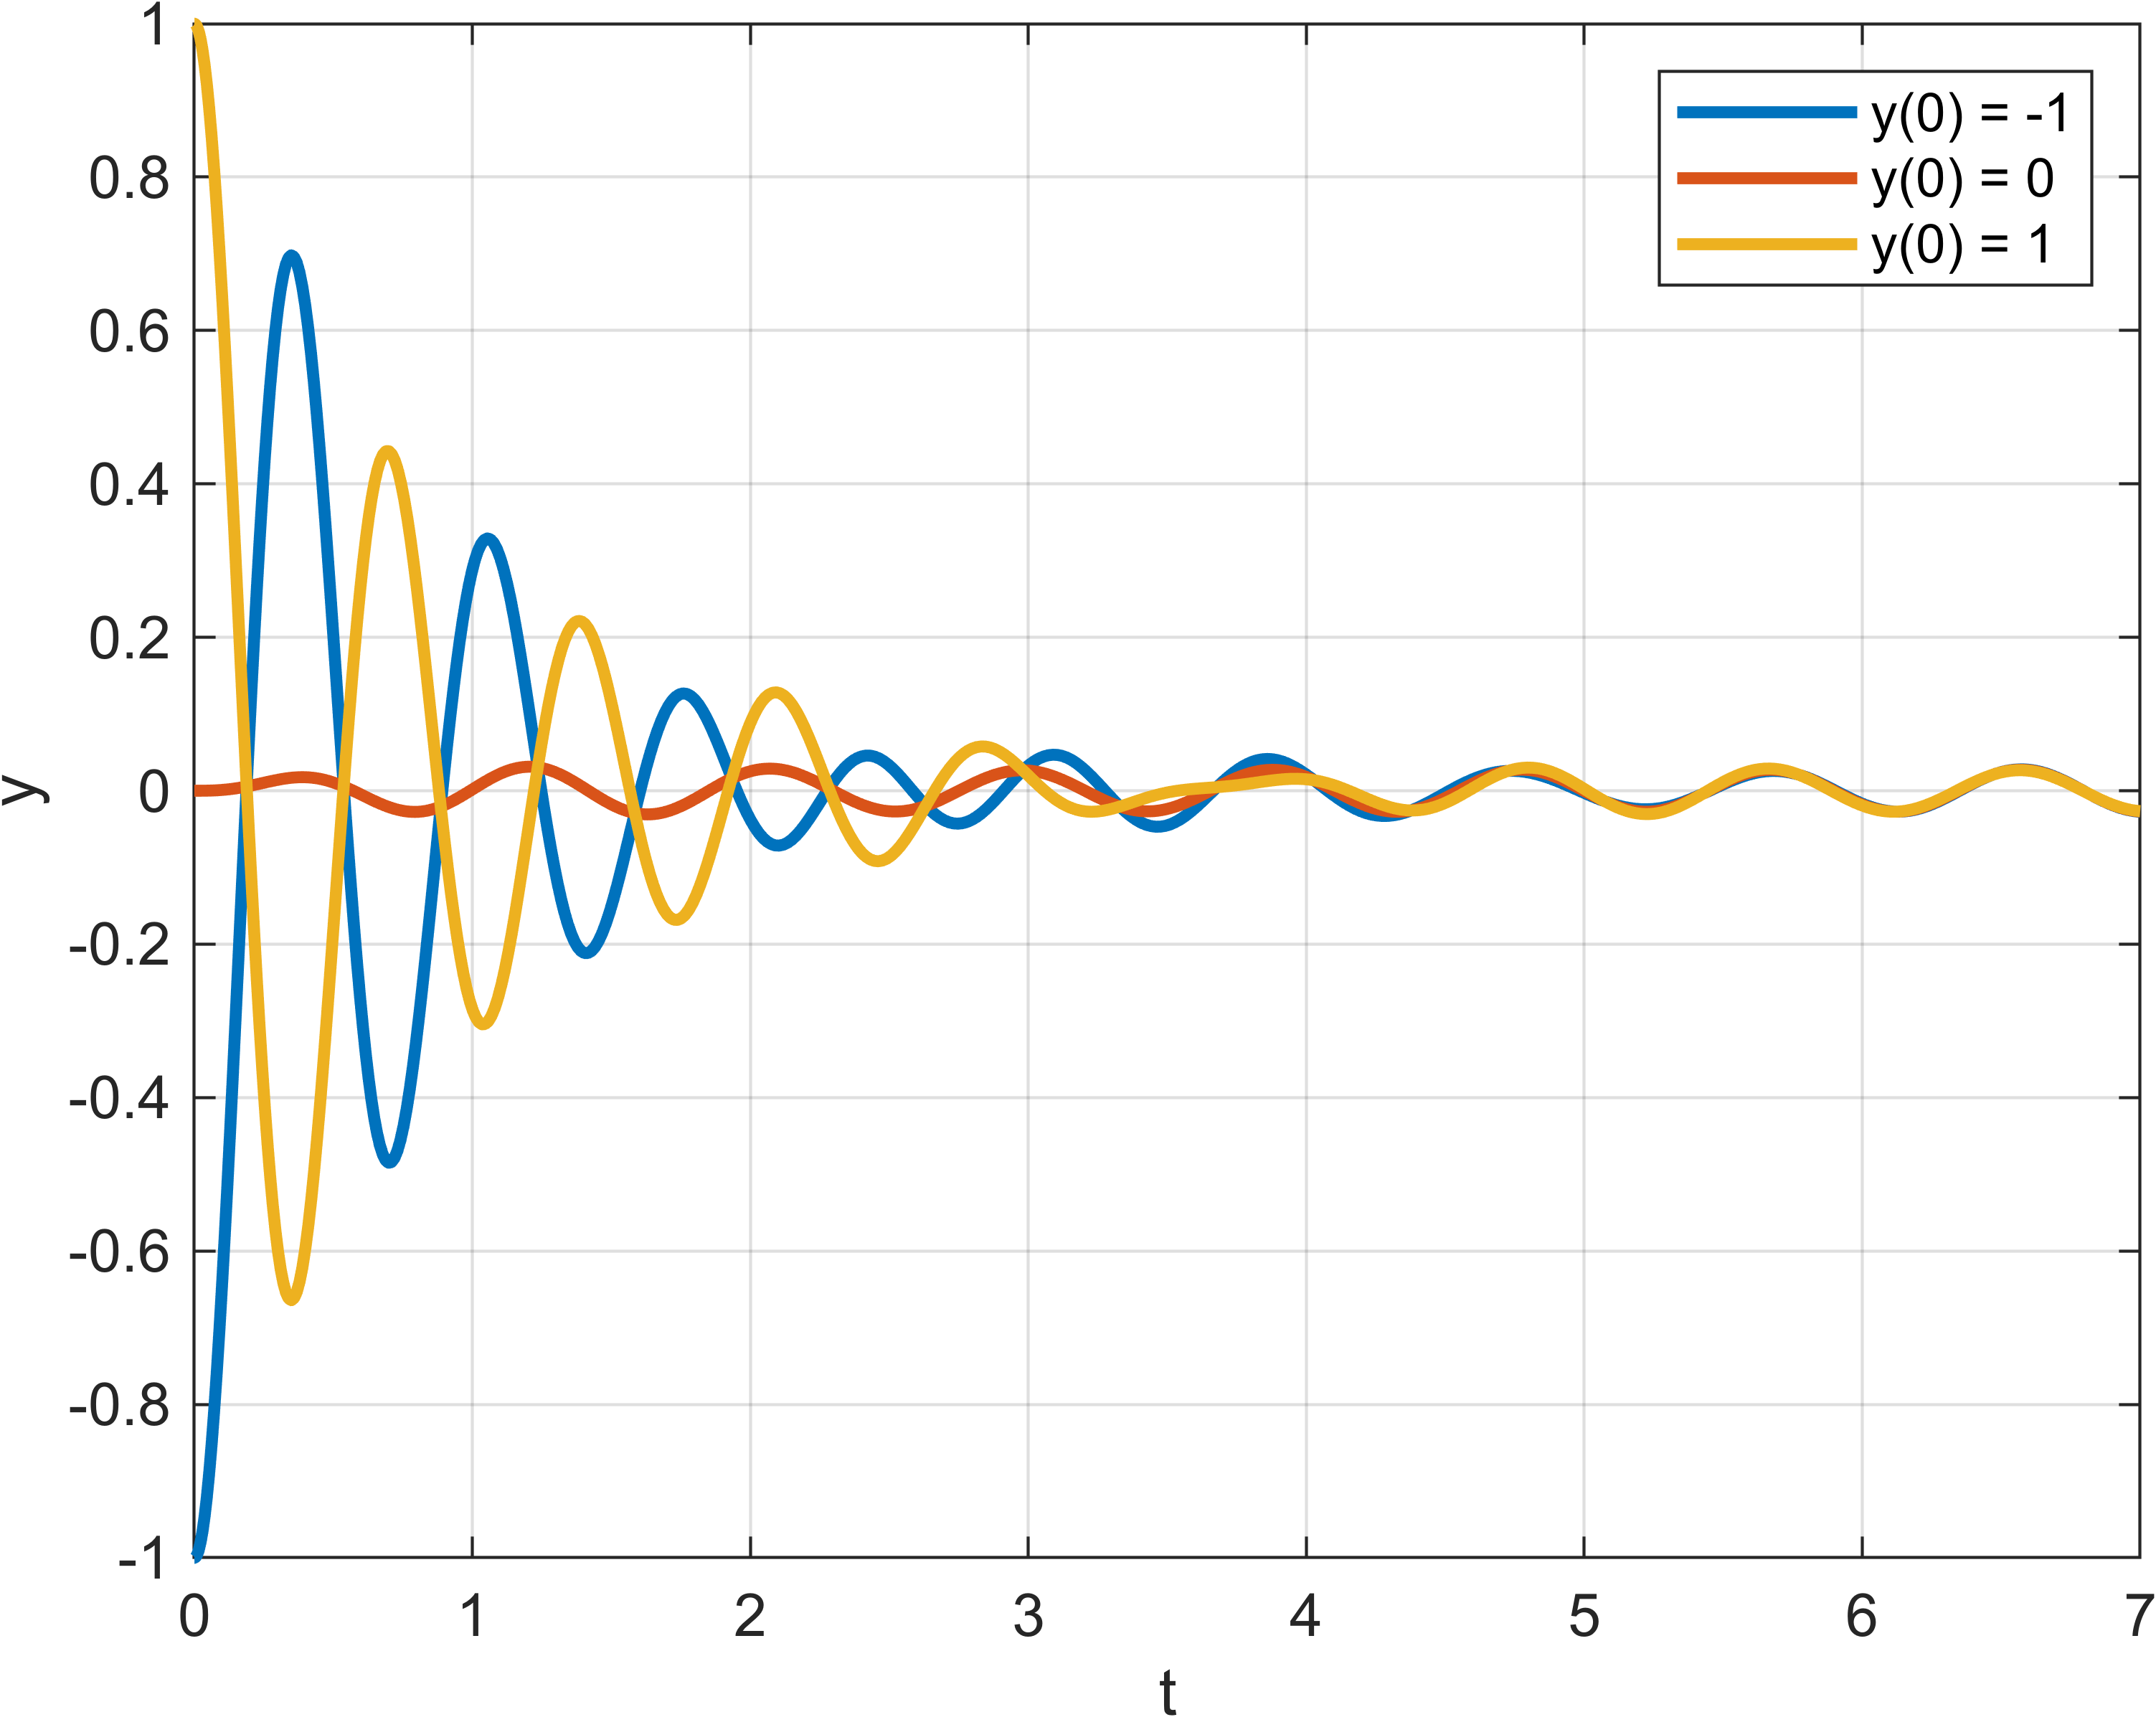
\includegraphics[width=0.7\textwidth, trim={0cm 0cm 0cm 0cm}]{../images/1_3.png}
    \caption{$u(t) = \sin(7t)$}
    \label{fig:1_3}
\end{figure}

\section{$a_0 = 81,\, a_1 = 0$}

\begin{figure}[ht]
    \centering
    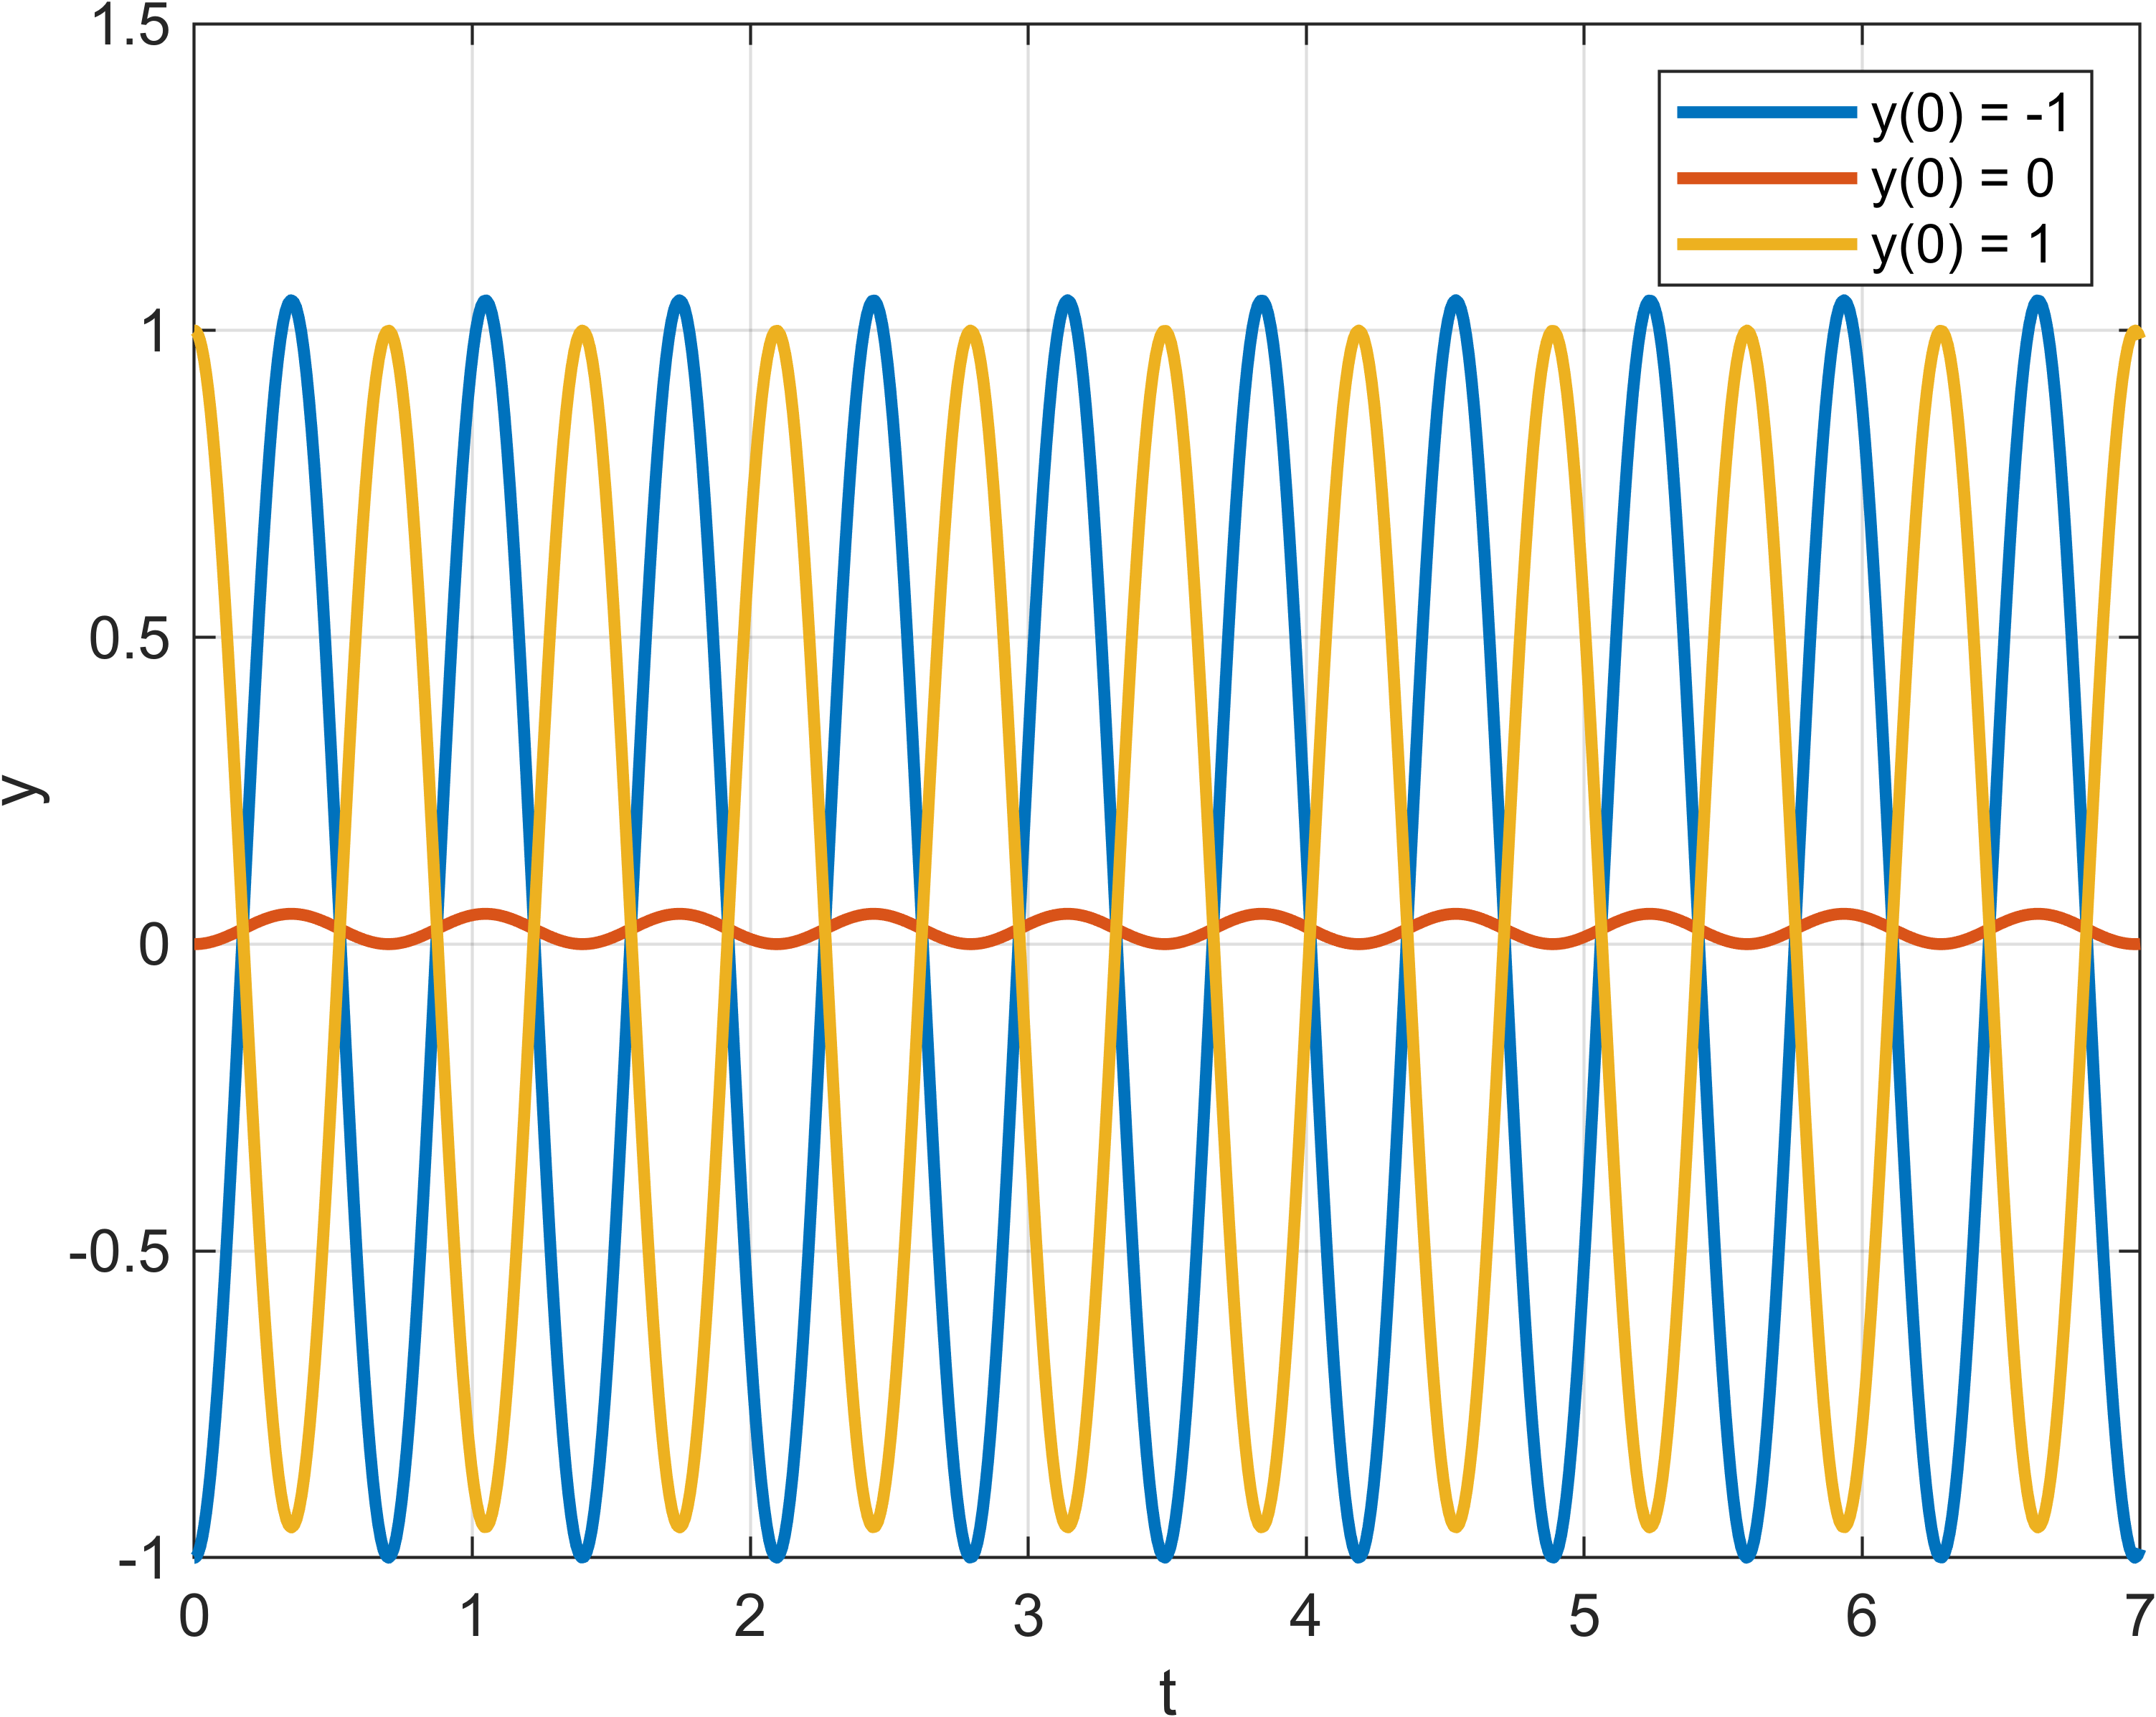
\includegraphics[width=0.7\textwidth, trim={0cm 0cm 0cm 0cm}]{../images/2_1.png}
    \caption{$u(t) = 2$}
    \label{fig:2_1}
\end{figure}

\begin{figure}[ht]
    \centering
    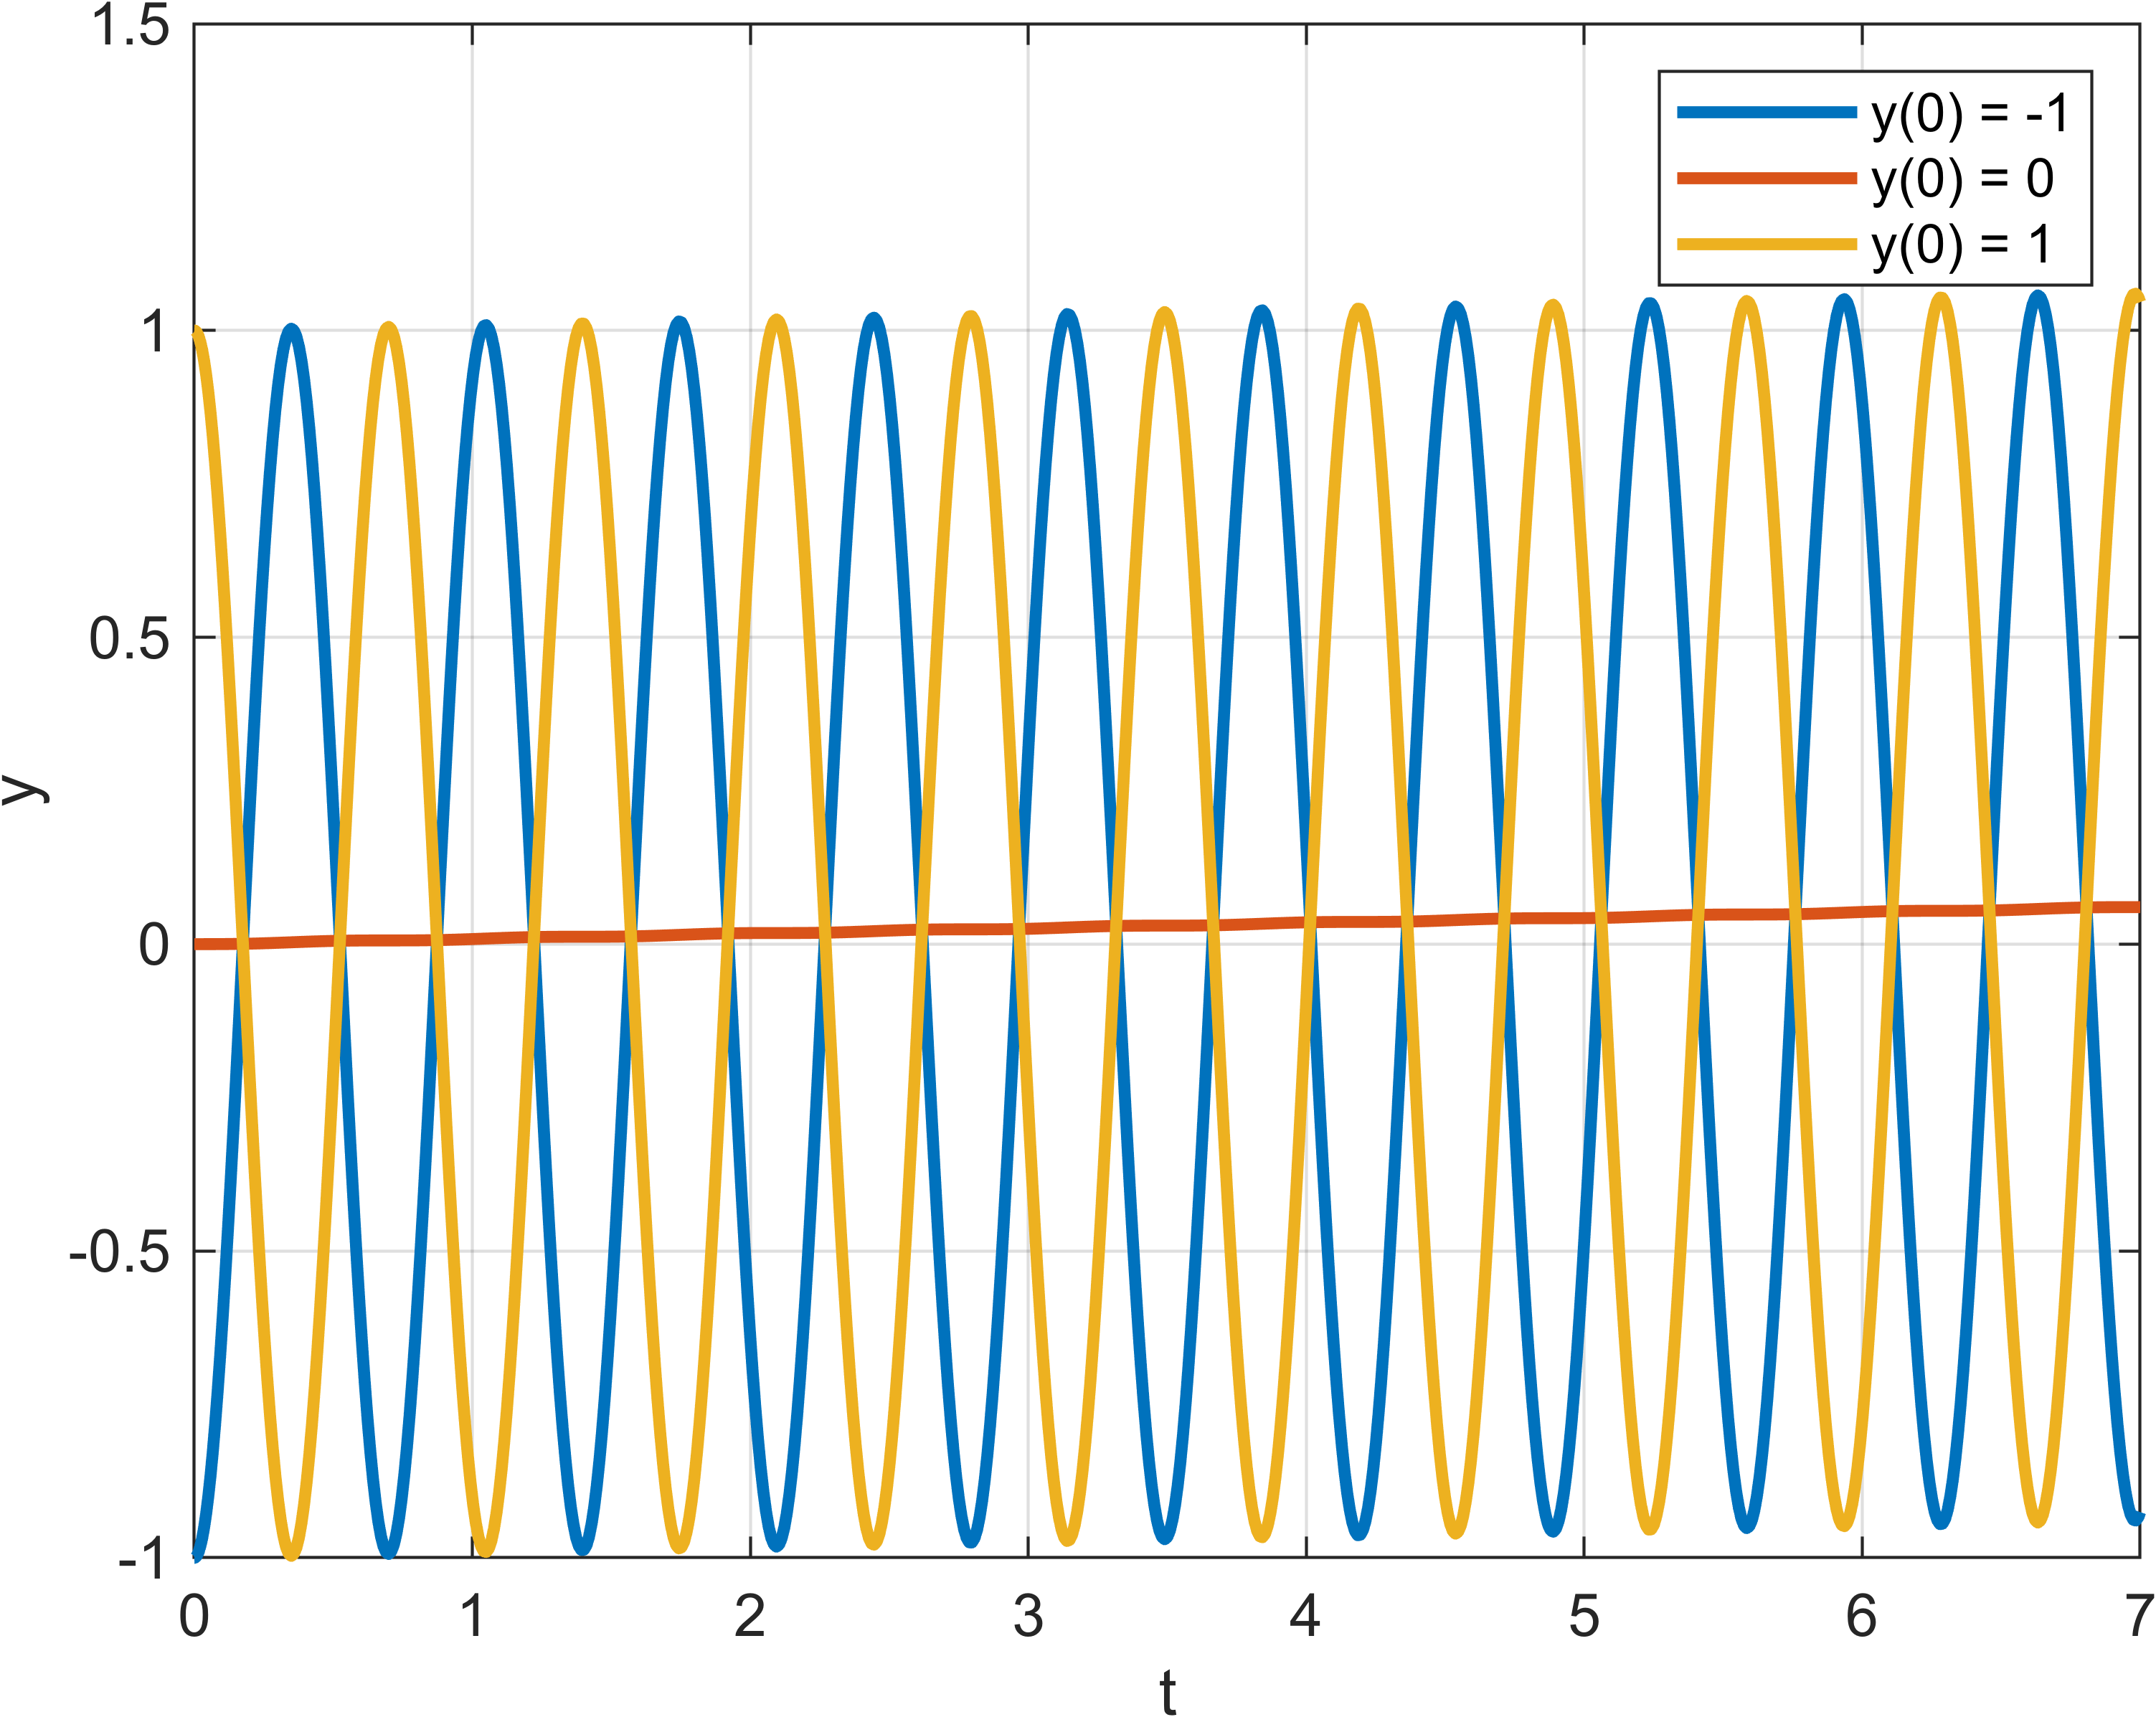
\includegraphics[width=0.7\textwidth, trim={0cm 0cm 0cm 0cm}]{../images/2_2.png}
    \caption{$u(t) = 0.7t$}
    \label{fig:2_2}
\end{figure}

\begin{figure}[ht]
    \centering
    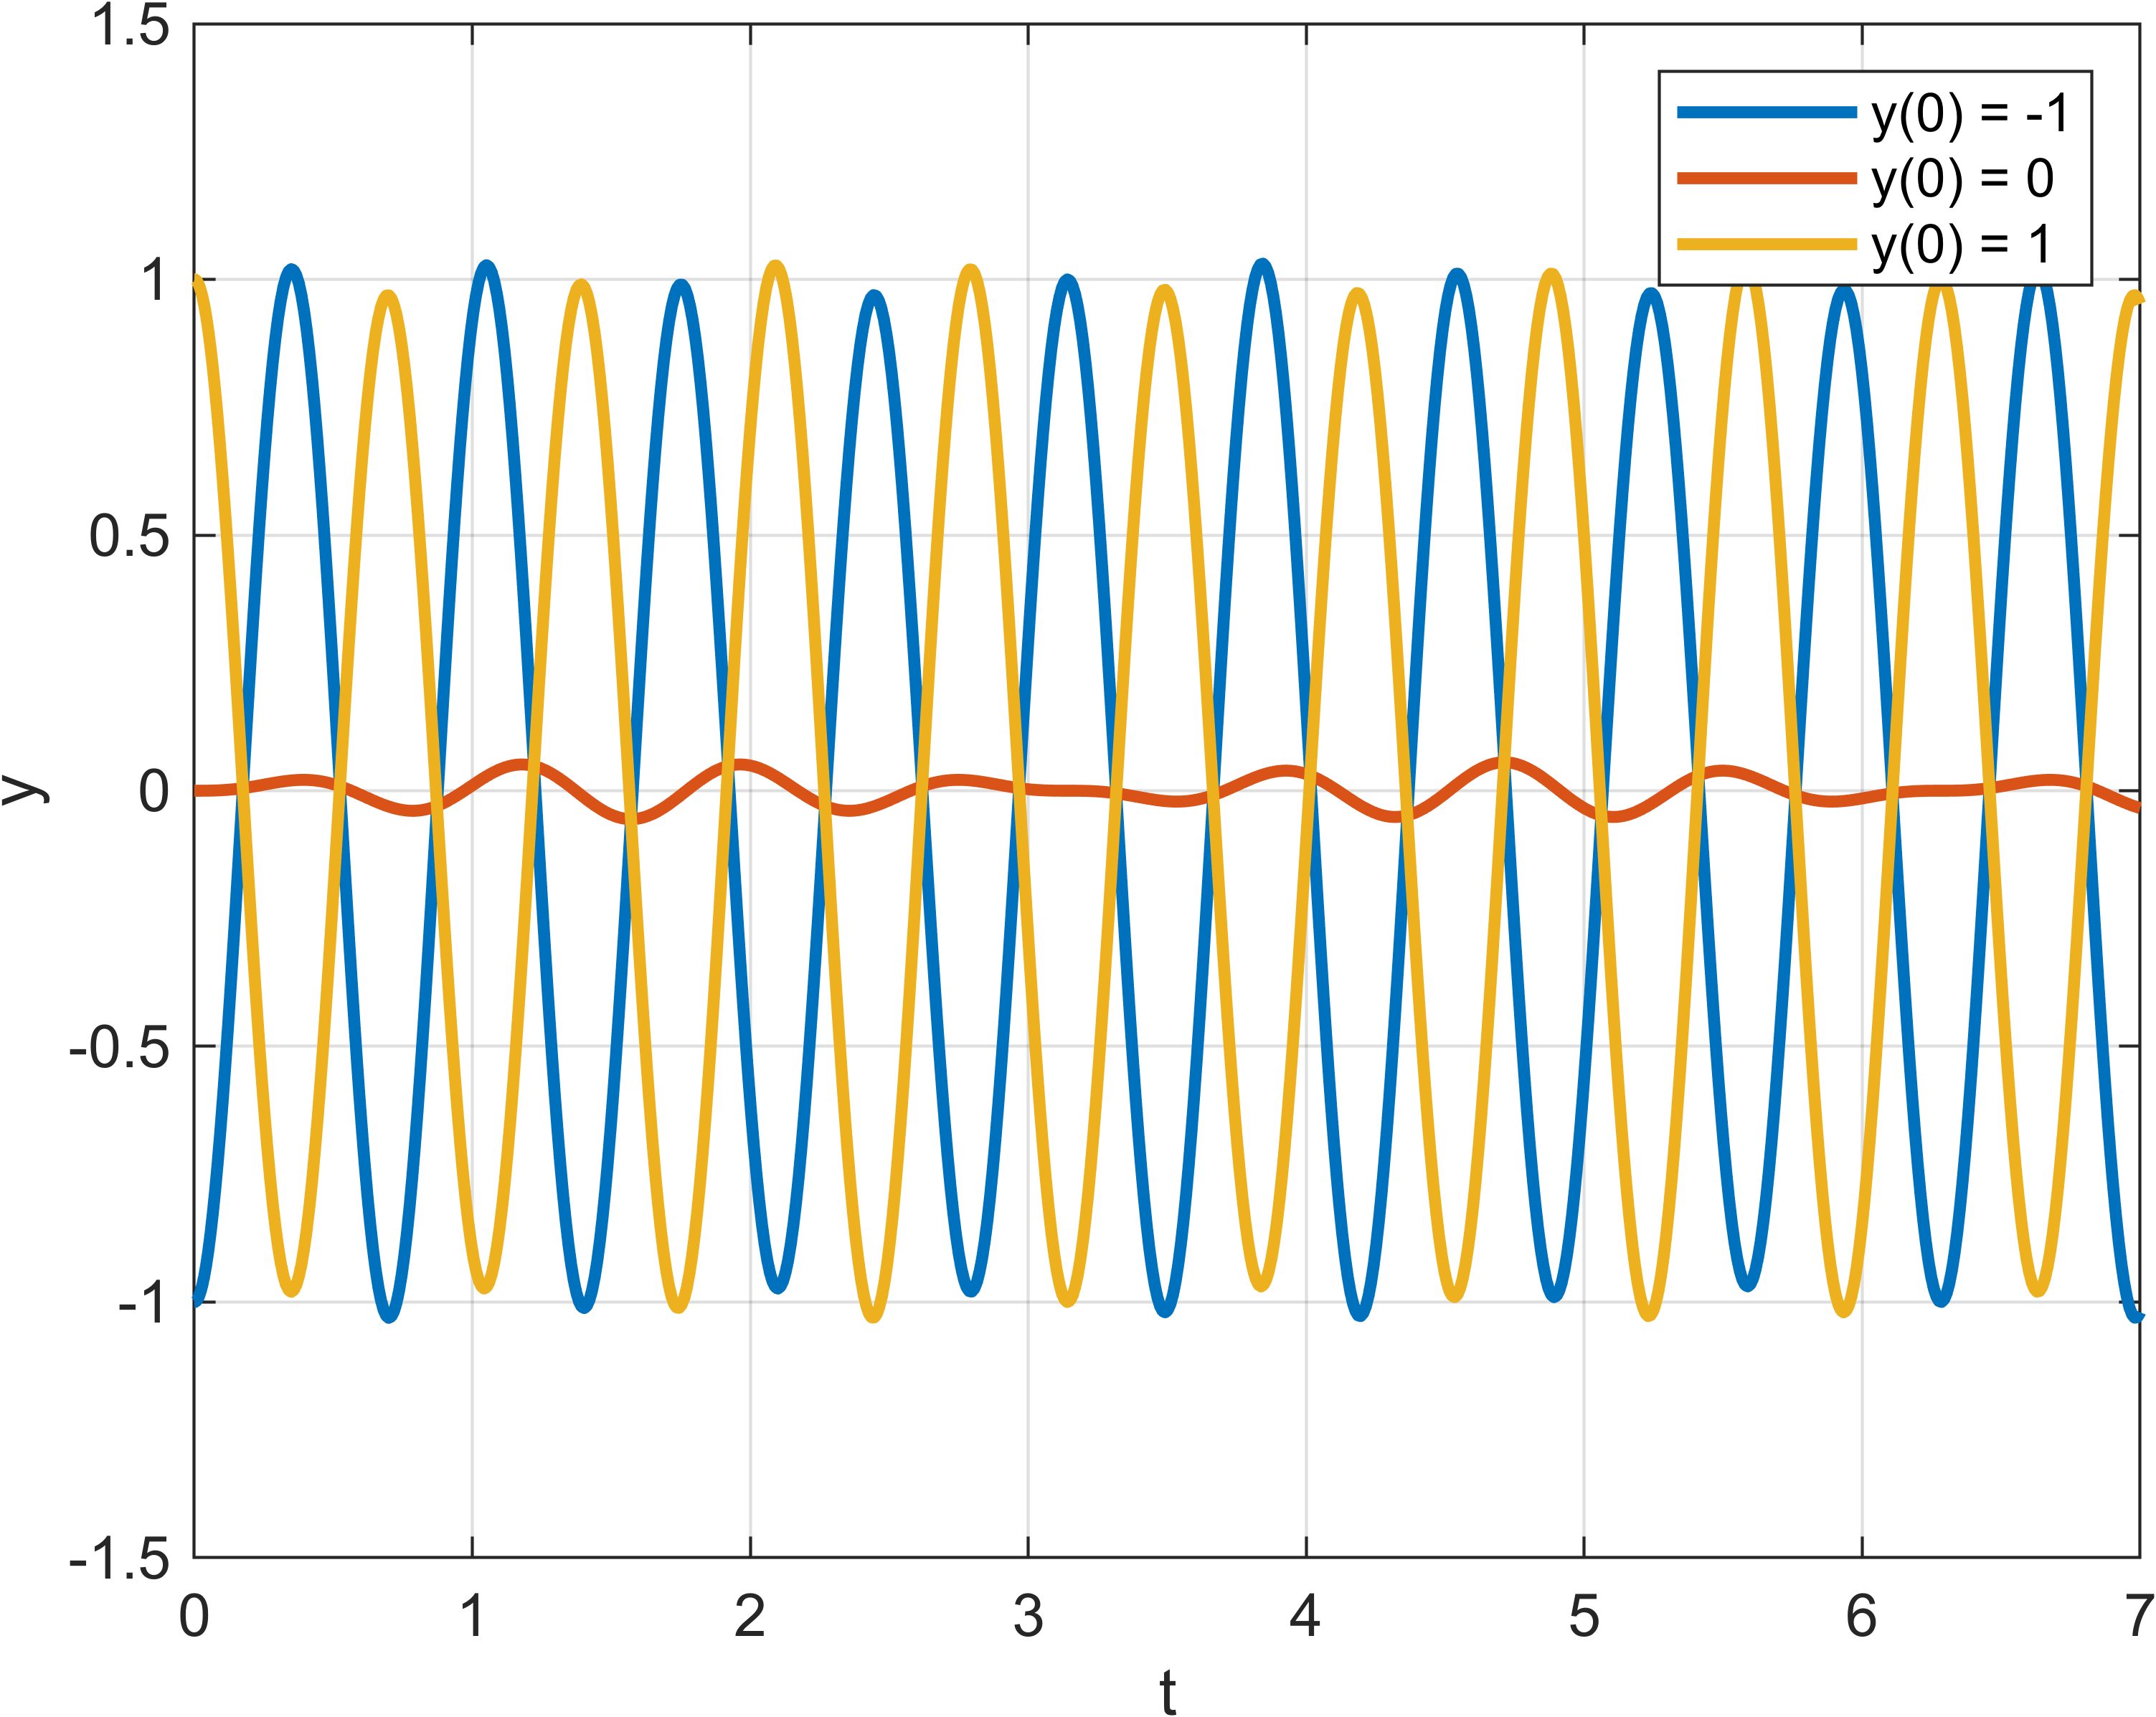
\includegraphics[width=0.7\textwidth, trim={0cm 0cm 0cm 0cm}]{../images/2_3.png}
    \caption{$u(t) = \sin(7t)$}
    \label{fig:2_3}
\end{figure}
 
\newpage
\section{$a_0 = 82.21,\, a_1 = -2.2$}
\begin{figure}[H]
    \centering
    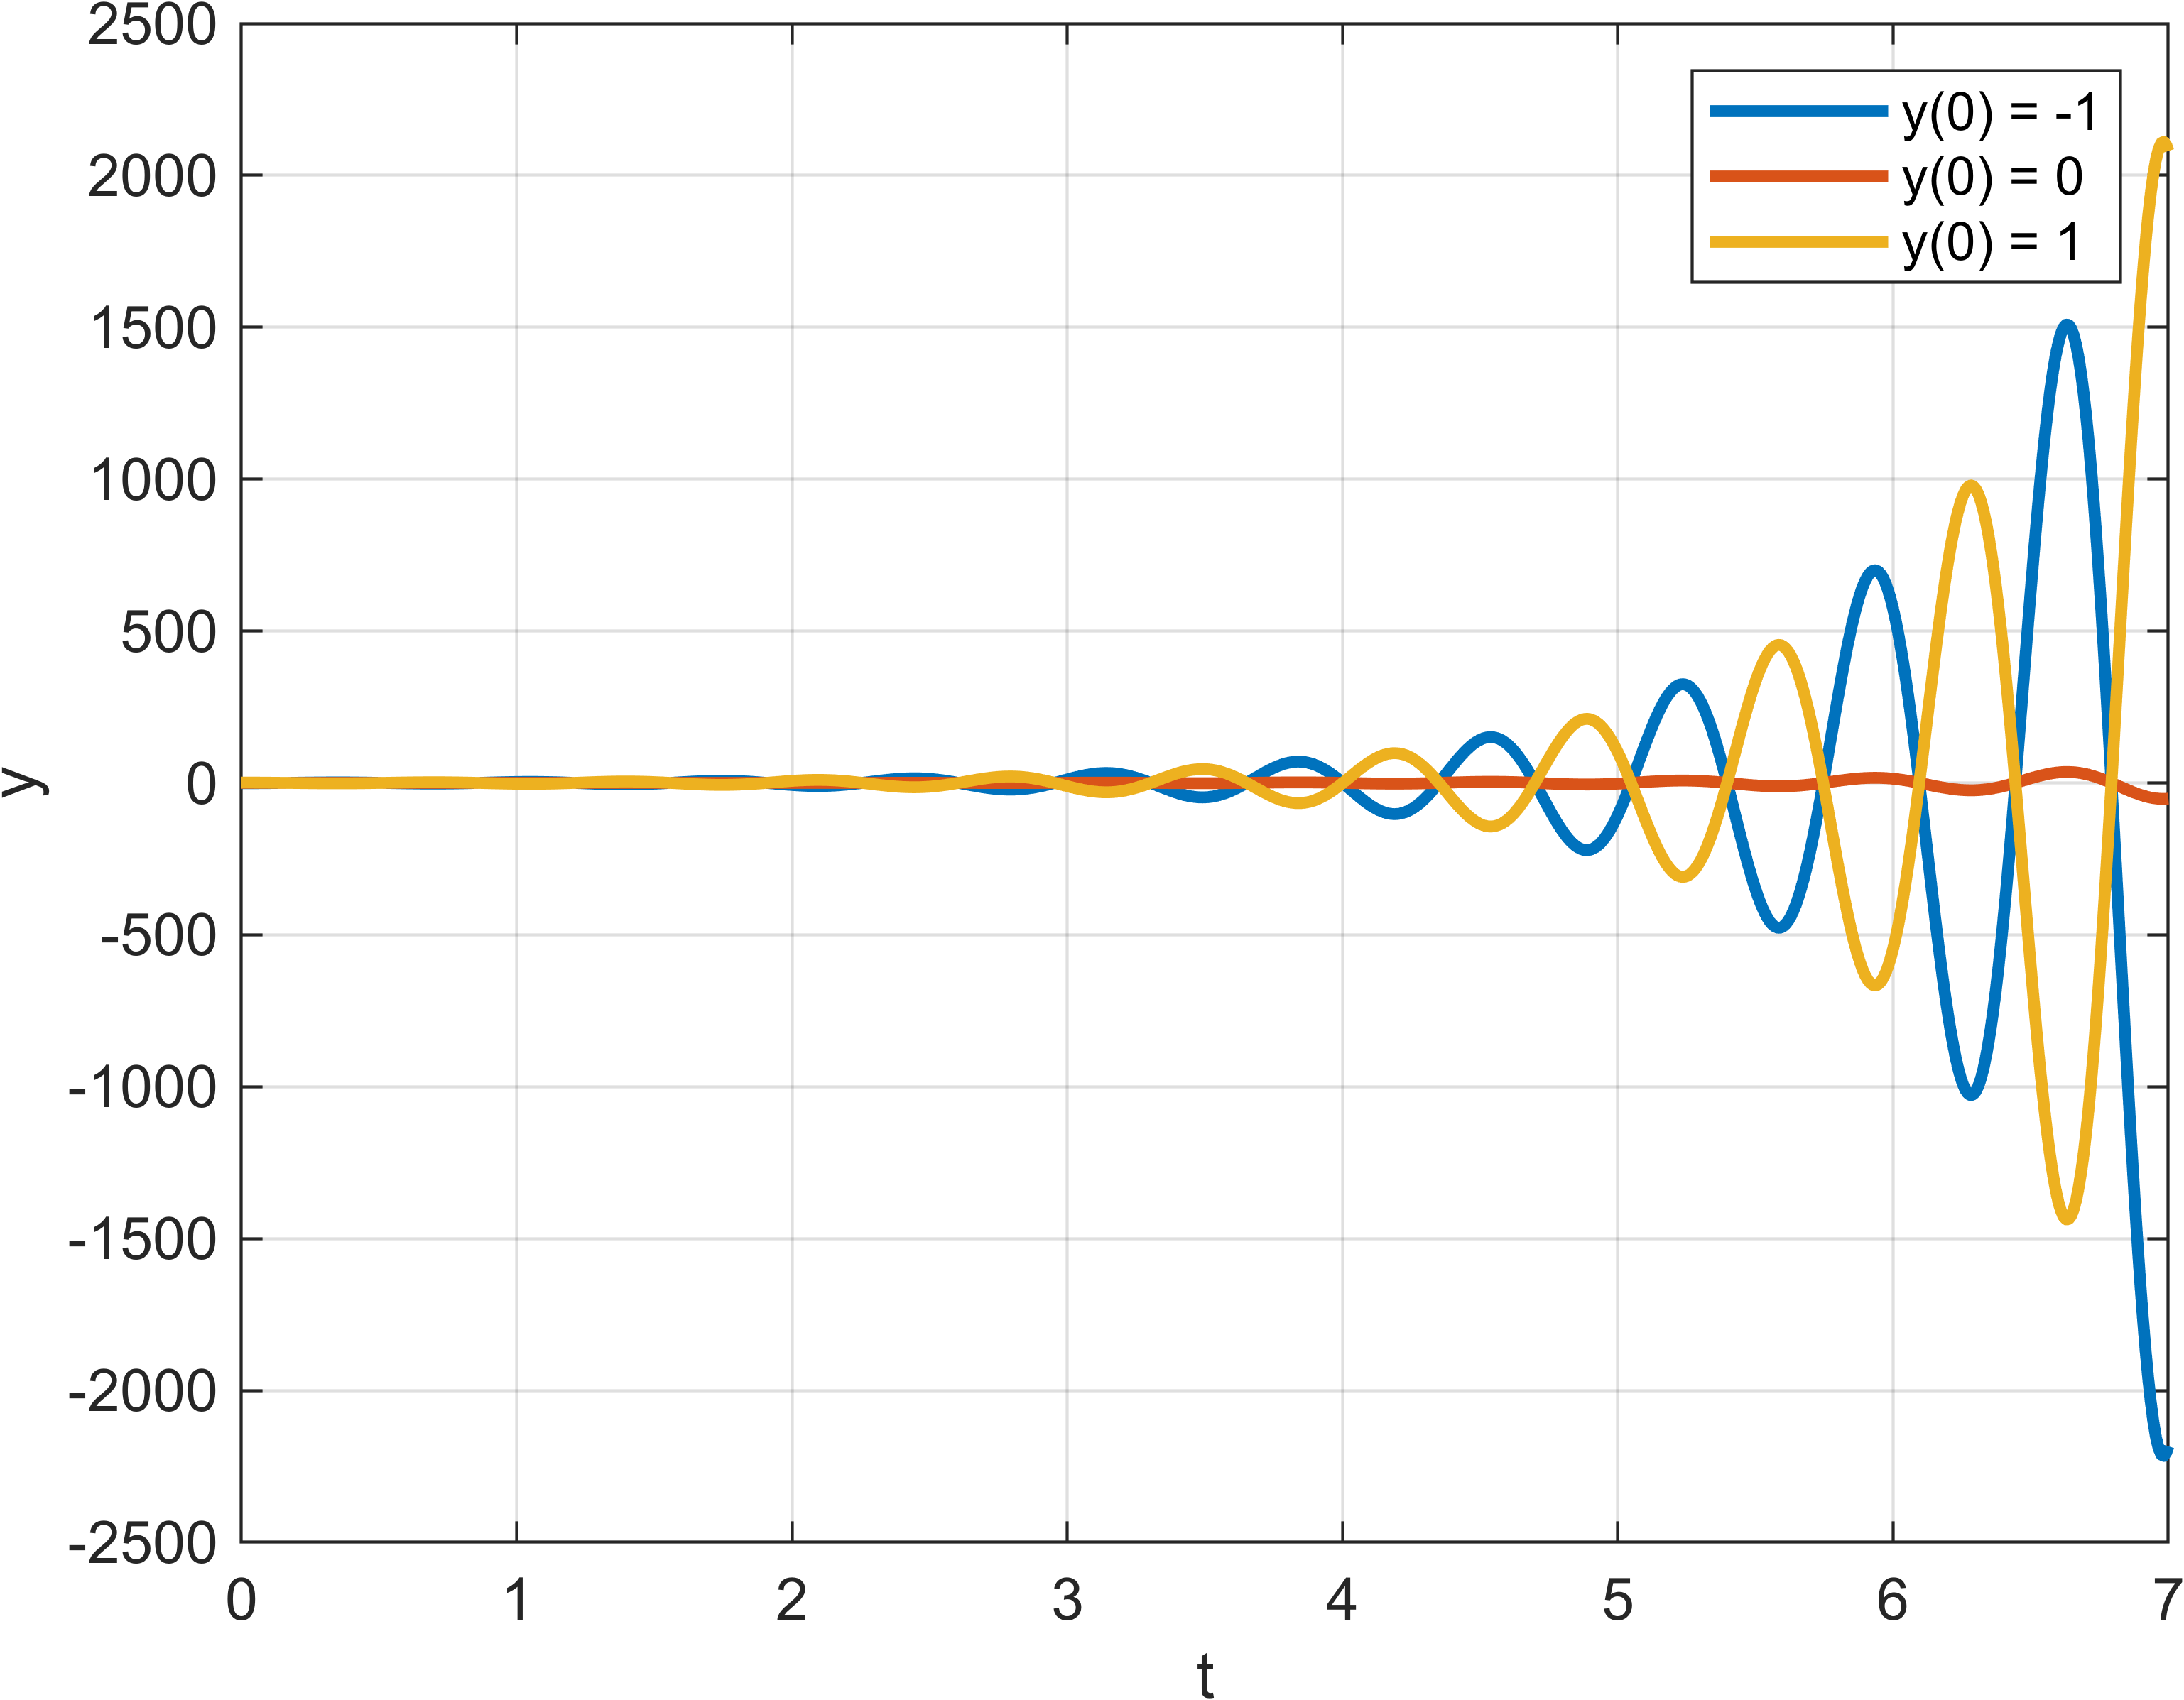
\includegraphics[width=0.7\textwidth, trim={0cm 0cm 0cm 0cm}]{../images/3_1.png}
    \caption{$u(t) = 2$}
    \label{fig:3_1}
\end{figure}

\begin{figure}[H]
    \centering
    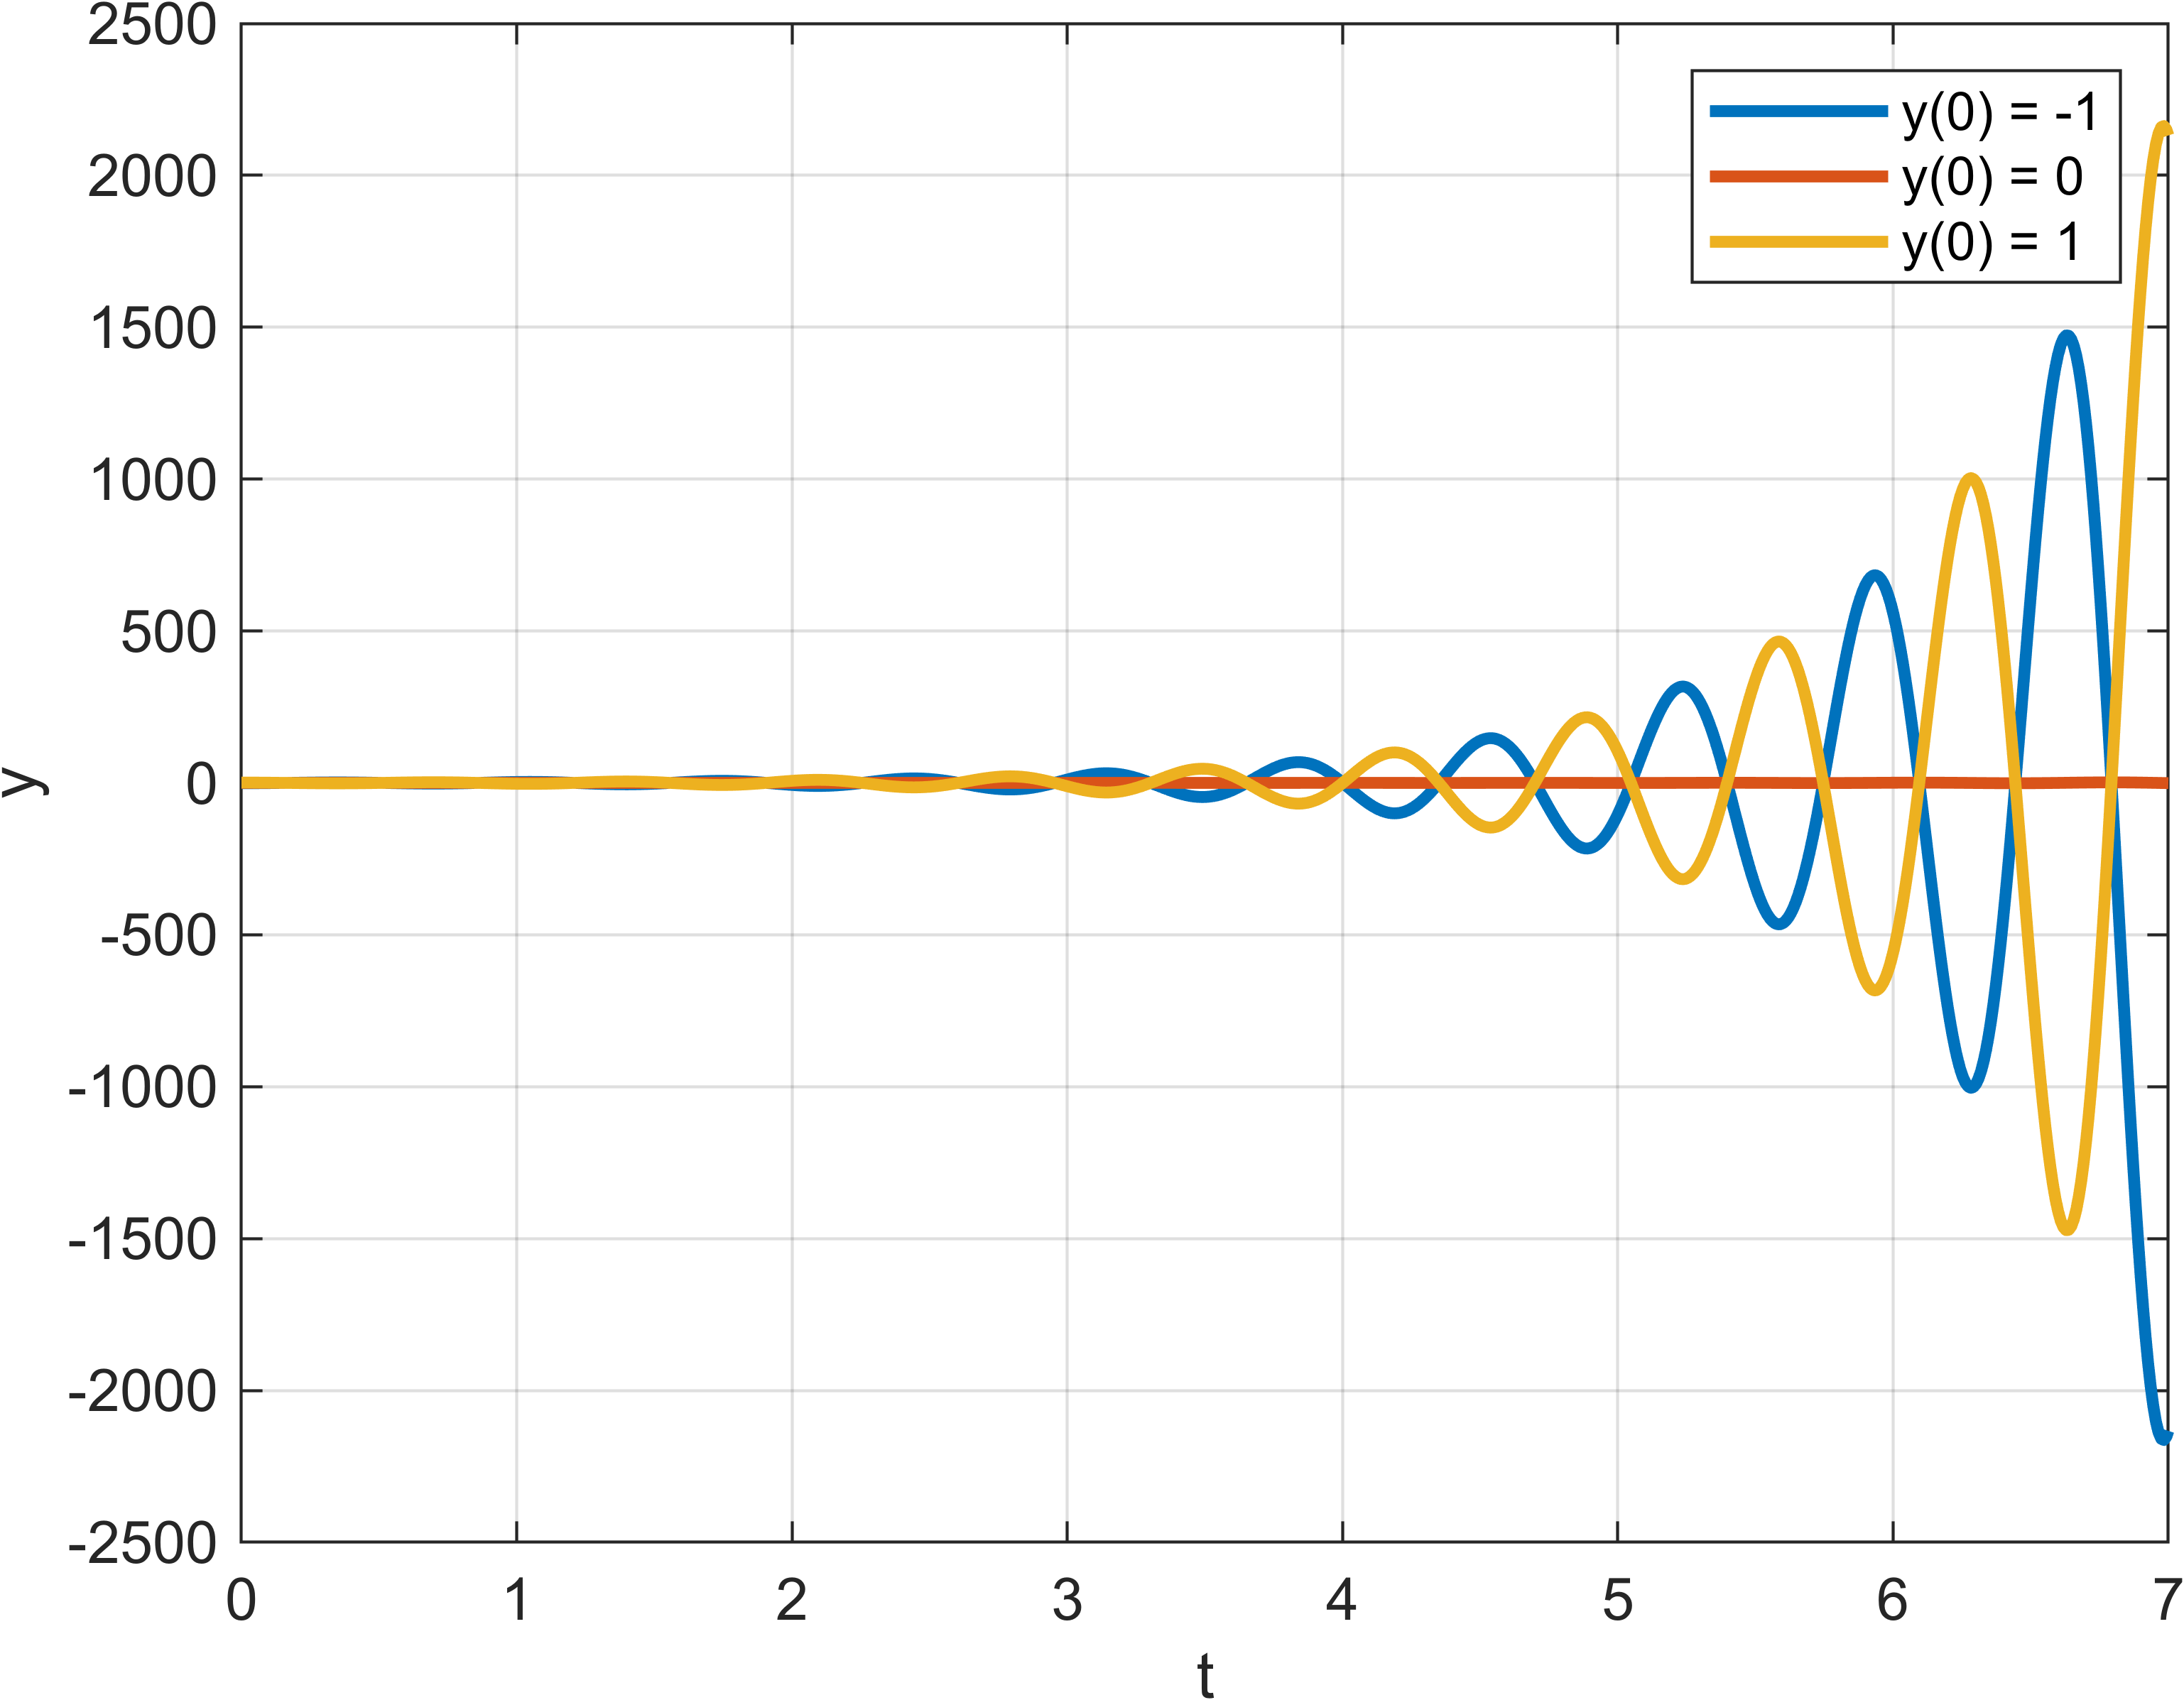
\includegraphics[width=0.7\textwidth, trim={0cm 0cm 0cm 0cm}]{../images/3_2.png}
    \caption{$u(t) = 0.7t$}
    \label{fig:3_2}
\end{figure}
 
\newpage
\begin{figure}[H]
    \centering
    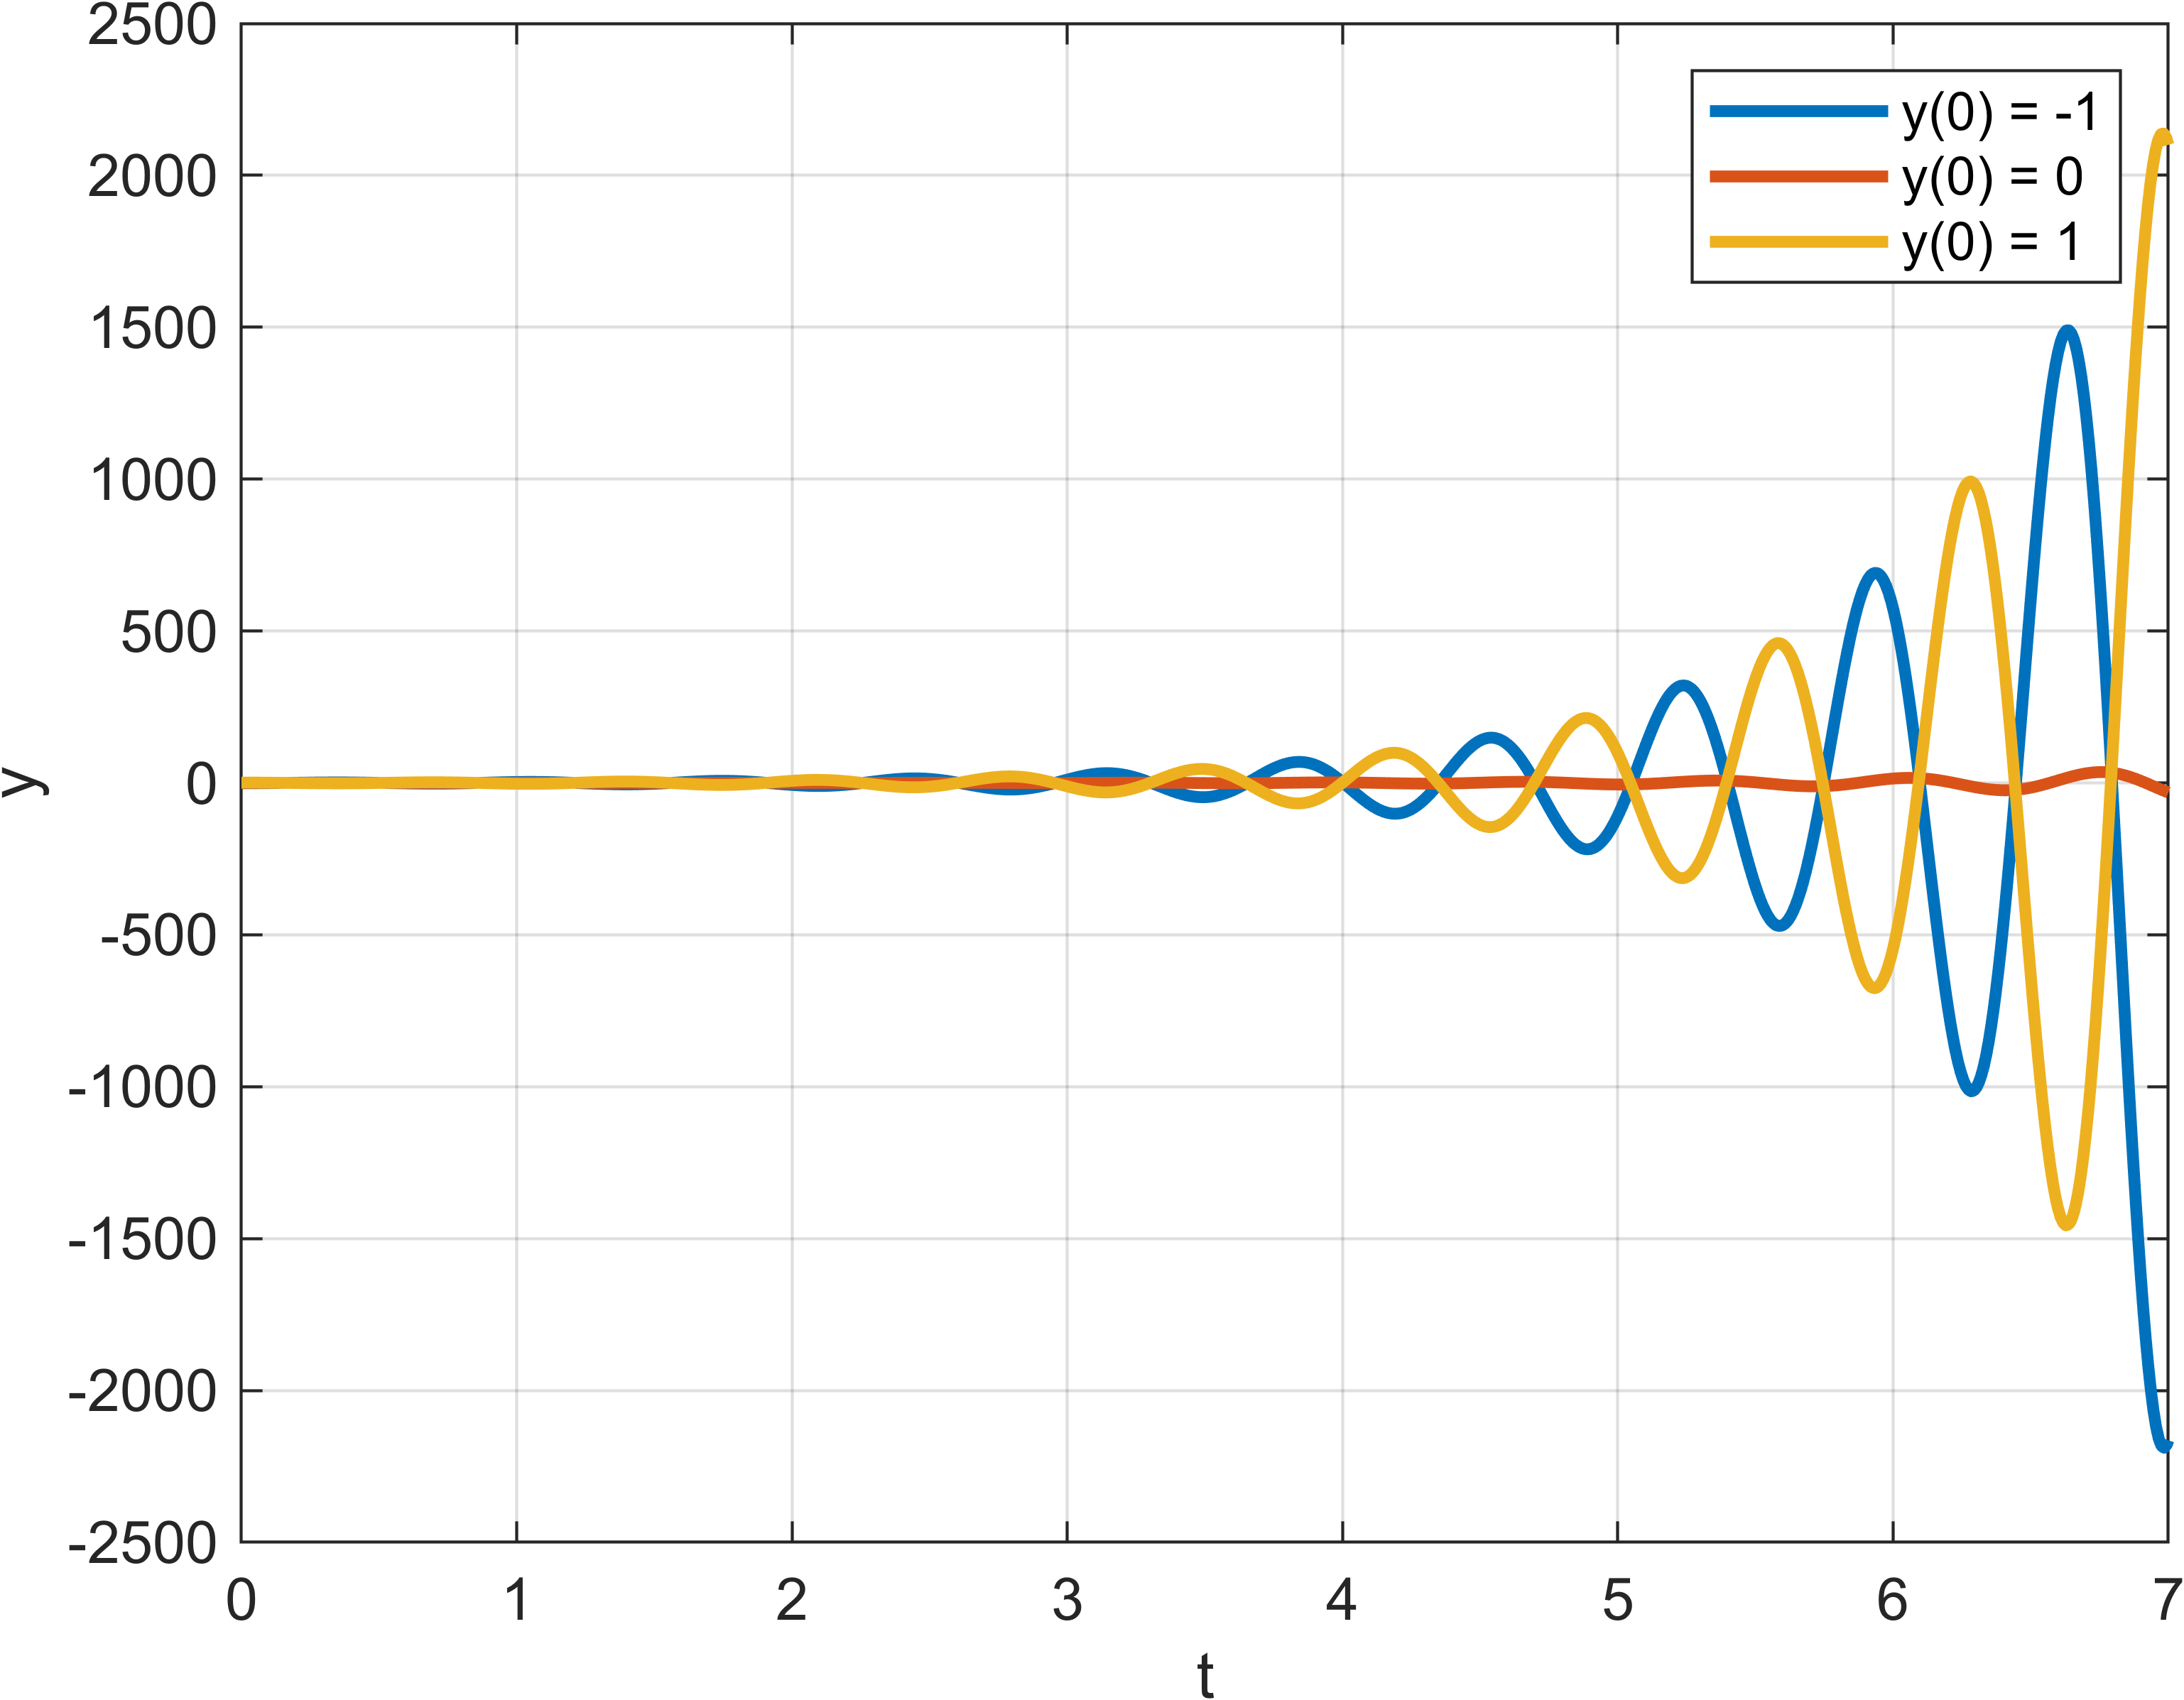
\includegraphics[width=0.7\textwidth, trim={0cm 0cm 0cm 0cm}]{../images/3_3.png}
    \caption{$u(t) = \sin(7t)$}
    \label{fig:3_3}
\end{figure}

Из графиков видно, что при подаче неконстантного входного сигнала, устойчивая система пытается сохранить 
устойчивость относительно нового входного сигнала. Система на границе устойчивости при достаточно больших начальных
условиях начинает колебаться около нового сигнала, но не уходит в неустойчивость. Неустойчивая система
при достаточно больших начальных условиях существенно не меняется при изменении входного сигнала из-за
превосходства неустойчивой составляющей над изменениями входного сигнала.
\endinput